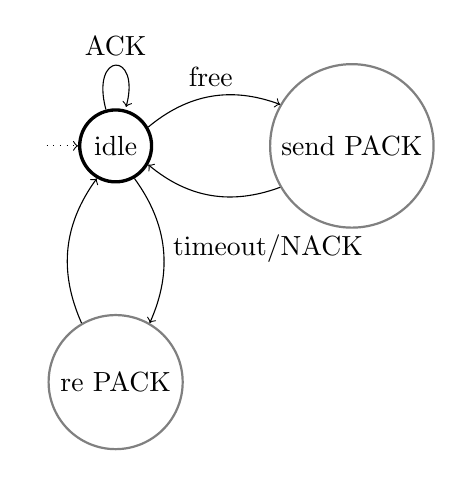
\begin{tikzpicture}
[
init/.style={circle, draw=black!100, very thick, minimum size=7mm,node distance=1cm},
state_split/.style={circle split, draw=gray!100, thick, minimum size=7mm,node distance=3cm},
state/.style={circle, draw=gray!100, thick, minimum size=7mm,node distance=3cm},
final/.style={circle, draw=black!60,  ultra thick, minimum size=10mm,node distance=23mm}
]
%Nodes
\node[init]     (start)                         {idle};
\node           (init)          [left of=start]     {};
\node[state]    (sack)          [right of=start]    {send PACK};
\node[state]    (reack)         [below of=start]    {re PACK};



%Lines
%\draw[->] (start.east) -- (synx.west);
%\draw[->] (synx.east) -- (end.west);
%\path[->] (start)  edge [loop above] node {a} (start); 
\draw[dotted, ->] (init.east) -- (start.west);
\path[->] 
          
(start) edge[bend left]         node[above]             {free}      (sack)
(sack)  edge[bend left]         node[below]             {}          (start)
(start) edge[bend left]         node[right]             {timeout/NACK} (reack)
(reack) edge[bend left]         node[left]              {}          (start)
(start) edge[loop above]        node[above]             {ACK}       (start);

\end{tikzpicture}